% Created by tikzDevice version 0.12.3.1 on 2021-10-16 07:50:32
% !TEX encoding = UTF-8 Unicode
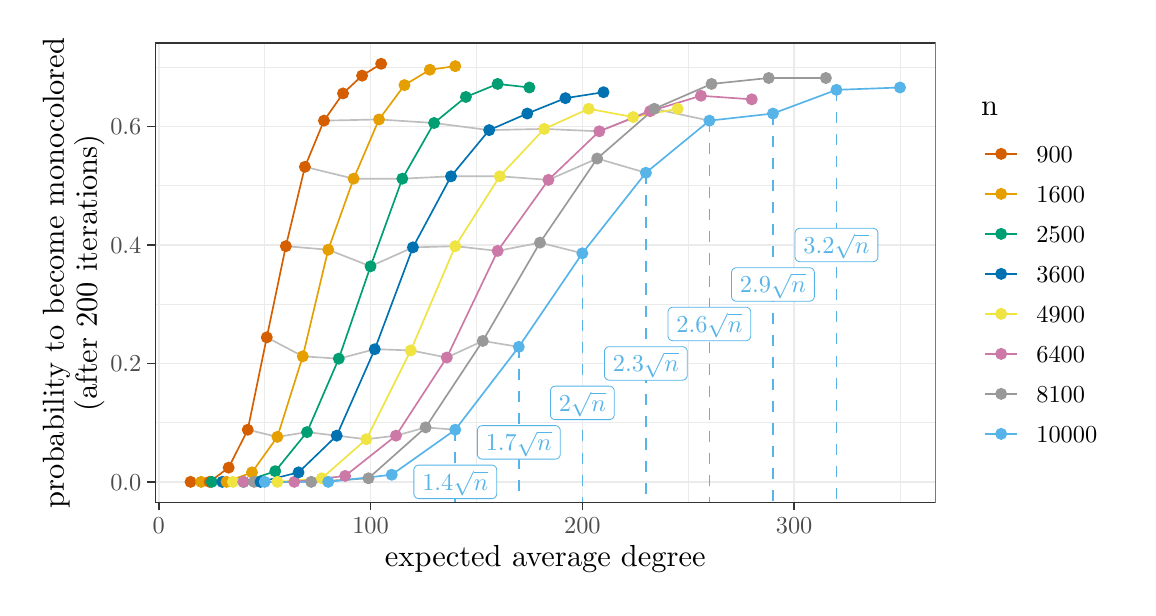
\begin{tikzpicture}[x=1pt,y=1pt]
\definecolor{fillColor}{RGB}{255,255,255}
\path[use as bounding box,fill=fillColor,fill opacity=0.00] (0,0) rectangle (397.48,202.36);
\begin{scope}
\path[clip] (  0.00,  0.00) rectangle (397.48,202.36);
\definecolor{drawColor}{RGB}{255,255,255}
\definecolor{fillColor}{RGB}{255,255,255}

\path[draw=drawColor,line width= 0.6pt,line join=round,line cap=round,fill=fillColor] (  0.00,  0.00) rectangle (397.48,202.36);
\end{scope}
\begin{scope}
\path[clip] ( 46.04, 30.69) rectangle (328.04,196.86);
\definecolor{fillColor}{RGB}{255,255,255}

\path[fill=fillColor] ( 46.04, 30.69) rectangle (328.04,196.86);
\definecolor{drawColor}{gray}{0.92}

\path[draw=drawColor,line width= 0.3pt,line join=round] ( 46.04, 59.64) --
	(328.04, 59.64);

\path[draw=drawColor,line width= 0.3pt,line join=round] ( 46.04,102.43) --
	(328.04,102.43);

\path[draw=drawColor,line width= 0.3pt,line join=round] ( 46.04,145.22) --
	(328.04,145.22);

\path[draw=drawColor,line width= 0.3pt,line join=round] ( 46.04,188.02) --
	(328.04,188.02);

\path[draw=drawColor,line width= 0.3pt,line join=round] ( 85.64, 30.69) --
	( 85.64,196.86);

\path[draw=drawColor,line width= 0.3pt,line join=round] (162.17, 30.69) --
	(162.17,196.86);

\path[draw=drawColor,line width= 0.3pt,line join=round] (238.69, 30.69) --
	(238.69,196.86);

\path[draw=drawColor,line width= 0.3pt,line join=round] (315.22, 30.69) --
	(315.22,196.86);

\path[draw=drawColor,line width= 0.6pt,line join=round] ( 46.04, 38.24) --
	(328.04, 38.24);

\path[draw=drawColor,line width= 0.6pt,line join=round] ( 46.04, 81.03) --
	(328.04, 81.03);

\path[draw=drawColor,line width= 0.6pt,line join=round] ( 46.04,123.83) --
	(328.04,123.83);

\path[draw=drawColor,line width= 0.6pt,line join=round] ( 46.04,166.62) --
	(328.04,166.62);

\path[draw=drawColor,line width= 0.6pt,line join=round] ( 47.38, 30.69) --
	( 47.38,196.86);

\path[draw=drawColor,line width= 0.6pt,line join=round] (123.90, 30.69) --
	(123.90,196.86);

\path[draw=drawColor,line width= 0.6pt,line join=round] (200.43, 30.69) --
	(200.43,196.86);

\path[draw=drawColor,line width= 0.6pt,line join=round] (276.95, 30.69) --
	(276.95,196.86);
\definecolor{drawColor}{RGB}{190,190,190}

\path[draw=drawColor,line width= 0.6pt,line join=round] ( 79.52, 57.07) --
	( 90.23, 54.50) --
	(100.94, 56.21) --
	(111.66, 54.93) --
	(122.37, 53.64) --
	(133.08, 54.93) --
	(143.80, 57.92) --
	(154.51, 57.07);

\path[draw=drawColor,line width= 0.6pt,line join=round] ( 86.40, 90.45) --
	( 99.41, 83.60) --
	(112.42, 82.75) --
	(125.43, 86.17) --
	(138.44, 85.74) --
	(151.45, 83.17) --
	(164.46, 89.16) --
	(177.47, 87.02);

\path[draw=drawColor,line width= 0.6pt,line join=round] ( 93.29,123.40) --
	(108.60,122.12) --
	(123.90,116.12) --
	(139.21,122.97) --
	(154.51,123.40) --
	(169.82,121.69) --
	(185.12,124.68) --
	(200.43,120.83);

\path[draw=drawColor,line width= 0.6pt,line join=round] (100.18,152.07) --
	(117.78,147.79) --
	(135.38,147.79) --
	(152.98,148.65) --
	(170.58,148.65) --
	(188.18,147.36) --
	(205.79,155.07) --
	(223.39,149.93);

\path[draw=drawColor,line width= 0.6pt,line join=round] (107.07,168.76) --
	(126.96,169.19) --
	(146.86,167.91) --
	(166.76,165.34) --
	(186.65,165.77) --
	(206.55,164.91) --
	(226.45,173.04) --
	(246.34,168.76);
\definecolor{drawColor}{RGB}{213,94,0}

\path[draw=drawColor,line width= 0.6pt,line join=round] ( 58.85, 38.24) --
	( 65.74, 38.24) --
	( 72.63, 43.37) --
	( 79.52, 57.07) --
	( 86.40, 90.45) --
	( 93.29,123.40) --
	(100.18,152.07) --
	(107.07,168.76) --
	(113.95,178.60) --
	(120.84,185.02) --
	(127.73,189.30);
\definecolor{drawColor}{RGB}{230,159,0}

\path[draw=drawColor,line width= 0.6pt,line join=round] ( 62.68, 38.24) --
	( 71.86, 38.24) --
	( 81.05, 41.66) --
	( 90.23, 54.50) --
	( 99.41, 83.60) --
	(108.60,122.12) --
	(117.78,147.79) --
	(126.96,169.19) --
	(136.15,181.60) --
	(145.33,187.16) --
	(154.51,188.45);
\definecolor{drawColor}{RGB}{0,158,115}

\path[draw=drawColor,line width= 0.6pt,line join=round] ( 66.51, 38.24) --
	( 77.99, 38.24) --
	( 89.46, 42.09) --
	(100.94, 56.21) --
	(112.42, 82.75) --
	(123.90,116.12) --
	(135.38,147.79) --
	(146.86,167.91) --
	(158.34,177.32) --
	(169.82,182.03) --
	(181.30,180.74);
\definecolor{drawColor}{RGB}{0,114,178}

\path[draw=drawColor,line width= 0.6pt,line join=round] ( 70.33, 38.24) --
	( 84.11, 38.24) --
	( 97.88, 41.66) --
	(111.66, 54.93) --
	(125.43, 86.17) --
	(139.21,122.97) --
	(152.98,148.65) --
	(166.76,165.34) --
	(180.53,171.33) --
	(194.31,176.89) --
	(208.08,179.03);
\definecolor{drawColor}{RGB}{240,228,66}

\path[draw=drawColor,line width= 0.6pt,line join=round] ( 74.16, 38.24) --
	( 90.23, 38.24) --
	(106.30, 39.52) --
	(122.37, 53.64) --
	(138.44, 85.74) --
	(154.51,123.40) --
	(170.58,148.65) --
	(186.65,165.77) --
	(202.72,173.04) --
	(218.79,170.05) --
	(234.87,173.04);
\definecolor{drawColor}{RGB}{204,121,167}

\path[draw=drawColor,line width= 0.6pt,line join=round] ( 77.99, 38.24) --
	( 96.35, 38.24) --
	(114.72, 40.38) --
	(133.08, 54.93) --
	(151.45, 83.17) --
	(169.82,121.69) --
	(188.18,147.36) --
	(206.55,164.91) --
	(224.92,172.19) --
	(243.28,177.75) --
	(261.65,176.46);
\definecolor{drawColor}{gray}{0.60}

\path[draw=drawColor,line width= 0.6pt,line join=round] ( 81.81, 38.24) --
	(102.47, 38.24) --
	(123.14, 39.52) --
	(143.80, 57.92) --
	(164.46, 89.16) --
	(185.12,124.68) --
	(205.79,155.07) --
	(226.45,173.04) --
	(247.11,182.03) --
	(267.77,184.17) --
	(288.43,184.17);
\definecolor{drawColor}{RGB}{86,180,233}

\path[draw=drawColor,line width= 0.6pt,line join=round] ( 85.64, 38.24) --
	(108.60, 38.24) --
	(131.55, 40.81) --
	(154.51, 57.07) --
	(177.47, 87.02) --
	(200.43,120.83) --
	(223.39,149.93) --
	(246.34,168.76) --
	(269.30,171.33) --
	(292.26,179.89) --
	(315.22,180.74);
\definecolor{drawColor}{RGB}{213,94,0}
\definecolor{fillColor}{RGB}{213,94,0}

\path[draw=drawColor,line width= 0.4pt,line join=round,line cap=round,fill=fillColor] ( 58.85, 38.24) circle (  1.96);
\definecolor{drawColor}{RGB}{230,159,0}
\definecolor{fillColor}{RGB}{230,159,0}

\path[draw=drawColor,line width= 0.4pt,line join=round,line cap=round,fill=fillColor] ( 62.68, 38.24) circle (  1.96);
\definecolor{drawColor}{RGB}{213,94,0}
\definecolor{fillColor}{RGB}{213,94,0}

\path[draw=drawColor,line width= 0.4pt,line join=round,line cap=round,fill=fillColor] ( 65.74, 38.24) circle (  1.96);
\definecolor{drawColor}{RGB}{0,158,115}
\definecolor{fillColor}{RGB}{0,158,115}

\path[draw=drawColor,line width= 0.4pt,line join=round,line cap=round,fill=fillColor] ( 66.51, 38.24) circle (  1.96);
\definecolor{drawColor}{RGB}{0,114,178}
\definecolor{fillColor}{RGB}{0,114,178}

\path[draw=drawColor,line width= 0.4pt,line join=round,line cap=round,fill=fillColor] ( 70.33, 38.24) circle (  1.96);
\definecolor{drawColor}{RGB}{230,159,0}
\definecolor{fillColor}{RGB}{230,159,0}

\path[draw=drawColor,line width= 0.4pt,line join=round,line cap=round,fill=fillColor] ( 71.86, 38.24) circle (  1.96);
\definecolor{drawColor}{RGB}{213,94,0}
\definecolor{fillColor}{RGB}{213,94,0}

\path[draw=drawColor,line width= 0.4pt,line join=round,line cap=round,fill=fillColor] ( 72.63, 43.37) circle (  1.96);
\definecolor{drawColor}{RGB}{240,228,66}
\definecolor{fillColor}{RGB}{240,228,66}

\path[draw=drawColor,line width= 0.4pt,line join=round,line cap=round,fill=fillColor] ( 74.16, 38.24) circle (  1.96);
\definecolor{drawColor}{RGB}{0,158,115}
\definecolor{fillColor}{RGB}{0,158,115}

\path[draw=drawColor,line width= 0.4pt,line join=round,line cap=round,fill=fillColor] ( 77.99, 38.24) circle (  1.96);
\definecolor{drawColor}{RGB}{204,121,167}
\definecolor{fillColor}{RGB}{204,121,167}

\path[draw=drawColor,line width= 0.4pt,line join=round,line cap=round,fill=fillColor] ( 77.99, 38.24) circle (  1.96);
\definecolor{drawColor}{RGB}{213,94,0}
\definecolor{fillColor}{RGB}{213,94,0}

\path[draw=drawColor,line width= 0.4pt,line join=round,line cap=round,fill=fillColor] ( 79.52, 57.07) circle (  1.96);
\definecolor{drawColor}{RGB}{230,159,0}
\definecolor{fillColor}{RGB}{230,159,0}

\path[draw=drawColor,line width= 0.4pt,line join=round,line cap=round,fill=fillColor] ( 81.05, 41.66) circle (  1.96);
\definecolor{drawColor}{gray}{0.60}
\definecolor{fillColor}{gray}{0.60}

\path[draw=drawColor,line width= 0.4pt,line join=round,line cap=round,fill=fillColor] ( 81.81, 38.24) circle (  1.96);
\definecolor{drawColor}{RGB}{0,114,178}
\definecolor{fillColor}{RGB}{0,114,178}

\path[draw=drawColor,line width= 0.4pt,line join=round,line cap=round,fill=fillColor] ( 84.11, 38.24) circle (  1.96);
\definecolor{drawColor}{RGB}{86,180,233}
\definecolor{fillColor}{RGB}{86,180,233}

\path[draw=drawColor,line width= 0.4pt,line join=round,line cap=round,fill=fillColor] ( 85.64, 38.24) circle (  1.96);
\definecolor{drawColor}{RGB}{213,94,0}
\definecolor{fillColor}{RGB}{213,94,0}

\path[draw=drawColor,line width= 0.4pt,line join=round,line cap=round,fill=fillColor] ( 86.40, 90.45) circle (  1.96);
\definecolor{drawColor}{RGB}{0,158,115}
\definecolor{fillColor}{RGB}{0,158,115}

\path[draw=drawColor,line width= 0.4pt,line join=round,line cap=round,fill=fillColor] ( 89.46, 42.09) circle (  1.96);
\definecolor{drawColor}{RGB}{230,159,0}
\definecolor{fillColor}{RGB}{230,159,0}

\path[draw=drawColor,line width= 0.4pt,line join=round,line cap=round,fill=fillColor] ( 90.23, 54.50) circle (  1.96);
\definecolor{drawColor}{RGB}{240,228,66}
\definecolor{fillColor}{RGB}{240,228,66}

\path[draw=drawColor,line width= 0.4pt,line join=round,line cap=round,fill=fillColor] ( 90.23, 38.24) circle (  1.96);
\definecolor{drawColor}{RGB}{213,94,0}
\definecolor{fillColor}{RGB}{213,94,0}

\path[draw=drawColor,line width= 0.4pt,line join=round,line cap=round,fill=fillColor] ( 93.29,123.40) circle (  1.96);
\definecolor{drawColor}{RGB}{204,121,167}
\definecolor{fillColor}{RGB}{204,121,167}

\path[draw=drawColor,line width= 0.4pt,line join=round,line cap=round,fill=fillColor] ( 96.35, 38.24) circle (  1.96);
\definecolor{drawColor}{RGB}{0,114,178}
\definecolor{fillColor}{RGB}{0,114,178}

\path[draw=drawColor,line width= 0.4pt,line join=round,line cap=round,fill=fillColor] ( 97.88, 41.66) circle (  1.96);
\definecolor{drawColor}{RGB}{230,159,0}
\definecolor{fillColor}{RGB}{230,159,0}

\path[draw=drawColor,line width= 0.4pt,line join=round,line cap=round,fill=fillColor] ( 99.41, 83.60) circle (  1.96);
\definecolor{drawColor}{RGB}{213,94,0}
\definecolor{fillColor}{RGB}{213,94,0}

\path[draw=drawColor,line width= 0.4pt,line join=round,line cap=round,fill=fillColor] (100.18,152.07) circle (  1.96);
\definecolor{drawColor}{RGB}{0,158,115}
\definecolor{fillColor}{RGB}{0,158,115}

\path[draw=drawColor,line width= 0.4pt,line join=round,line cap=round,fill=fillColor] (100.94, 56.21) circle (  1.96);
\definecolor{drawColor}{gray}{0.60}
\definecolor{fillColor}{gray}{0.60}

\path[draw=drawColor,line width= 0.4pt,line join=round,line cap=round,fill=fillColor] (102.47, 38.24) circle (  1.96);
\definecolor{drawColor}{RGB}{240,228,66}
\definecolor{fillColor}{RGB}{240,228,66}

\path[draw=drawColor,line width= 0.4pt,line join=round,line cap=round,fill=fillColor] (106.30, 39.52) circle (  1.96);
\definecolor{drawColor}{RGB}{213,94,0}
\definecolor{fillColor}{RGB}{213,94,0}

\path[draw=drawColor,line width= 0.4pt,line join=round,line cap=round,fill=fillColor] (107.07,168.76) circle (  1.96);
\definecolor{drawColor}{RGB}{230,159,0}
\definecolor{fillColor}{RGB}{230,159,0}

\path[draw=drawColor,line width= 0.4pt,line join=round,line cap=round,fill=fillColor] (108.60,122.12) circle (  1.96);
\definecolor{drawColor}{RGB}{86,180,233}
\definecolor{fillColor}{RGB}{86,180,233}

\path[draw=drawColor,line width= 0.4pt,line join=round,line cap=round,fill=fillColor] (108.60, 38.24) circle (  1.96);
\definecolor{drawColor}{RGB}{0,114,178}
\definecolor{fillColor}{RGB}{0,114,178}

\path[draw=drawColor,line width= 0.4pt,line join=round,line cap=round,fill=fillColor] (111.66, 54.93) circle (  1.96);
\definecolor{drawColor}{RGB}{0,158,115}
\definecolor{fillColor}{RGB}{0,158,115}

\path[draw=drawColor,line width= 0.4pt,line join=round,line cap=round,fill=fillColor] (112.42, 82.75) circle (  1.96);
\definecolor{drawColor}{RGB}{213,94,0}
\definecolor{fillColor}{RGB}{213,94,0}

\path[draw=drawColor,line width= 0.4pt,line join=round,line cap=round,fill=fillColor] (113.95,178.60) circle (  1.96);
\definecolor{drawColor}{RGB}{204,121,167}
\definecolor{fillColor}{RGB}{204,121,167}

\path[draw=drawColor,line width= 0.4pt,line join=round,line cap=round,fill=fillColor] (114.72, 40.38) circle (  1.96);
\definecolor{drawColor}{RGB}{230,159,0}
\definecolor{fillColor}{RGB}{230,159,0}

\path[draw=drawColor,line width= 0.4pt,line join=round,line cap=round,fill=fillColor] (117.78,147.79) circle (  1.96);
\definecolor{drawColor}{RGB}{213,94,0}
\definecolor{fillColor}{RGB}{213,94,0}

\path[draw=drawColor,line width= 0.4pt,line join=round,line cap=round,fill=fillColor] (120.84,185.02) circle (  1.96);
\definecolor{drawColor}{RGB}{240,228,66}
\definecolor{fillColor}{RGB}{240,228,66}

\path[draw=drawColor,line width= 0.4pt,line join=round,line cap=round,fill=fillColor] (122.37, 53.64) circle (  1.96);
\definecolor{drawColor}{gray}{0.60}
\definecolor{fillColor}{gray}{0.60}

\path[draw=drawColor,line width= 0.4pt,line join=round,line cap=round,fill=fillColor] (123.14, 39.52) circle (  1.96);
\definecolor{drawColor}{RGB}{0,158,115}
\definecolor{fillColor}{RGB}{0,158,115}

\path[draw=drawColor,line width= 0.4pt,line join=round,line cap=round,fill=fillColor] (123.90,116.12) circle (  1.96);
\definecolor{drawColor}{RGB}{0,114,178}
\definecolor{fillColor}{RGB}{0,114,178}

\path[draw=drawColor,line width= 0.4pt,line join=round,line cap=round,fill=fillColor] (125.43, 86.17) circle (  1.96);
\definecolor{drawColor}{RGB}{230,159,0}
\definecolor{fillColor}{RGB}{230,159,0}

\path[draw=drawColor,line width= 0.4pt,line join=round,line cap=round,fill=fillColor] (126.96,169.19) circle (  1.96);
\definecolor{drawColor}{RGB}{213,94,0}
\definecolor{fillColor}{RGB}{213,94,0}

\path[draw=drawColor,line width= 0.4pt,line join=round,line cap=round,fill=fillColor] (127.73,189.30) circle (  1.96);
\definecolor{drawColor}{RGB}{86,180,233}
\definecolor{fillColor}{RGB}{86,180,233}

\path[draw=drawColor,line width= 0.4pt,line join=round,line cap=round,fill=fillColor] (131.55, 40.81) circle (  1.96);
\definecolor{drawColor}{RGB}{204,121,167}
\definecolor{fillColor}{RGB}{204,121,167}

\path[draw=drawColor,line width= 0.4pt,line join=round,line cap=round,fill=fillColor] (133.08, 54.93) circle (  1.96);
\definecolor{drawColor}{RGB}{0,158,115}
\definecolor{fillColor}{RGB}{0,158,115}

\path[draw=drawColor,line width= 0.4pt,line join=round,line cap=round,fill=fillColor] (135.38,147.79) circle (  1.96);
\definecolor{drawColor}{RGB}{230,159,0}
\definecolor{fillColor}{RGB}{230,159,0}

\path[draw=drawColor,line width= 0.4pt,line join=round,line cap=round,fill=fillColor] (136.15,181.60) circle (  1.96);
\definecolor{drawColor}{RGB}{240,228,66}
\definecolor{fillColor}{RGB}{240,228,66}

\path[draw=drawColor,line width= 0.4pt,line join=round,line cap=round,fill=fillColor] (138.44, 85.74) circle (  1.96);
\definecolor{drawColor}{RGB}{0,114,178}
\definecolor{fillColor}{RGB}{0,114,178}

\path[draw=drawColor,line width= 0.4pt,line join=round,line cap=round,fill=fillColor] (139.21,122.97) circle (  1.96);
\definecolor{drawColor}{gray}{0.60}
\definecolor{fillColor}{gray}{0.60}

\path[draw=drawColor,line width= 0.4pt,line join=round,line cap=round,fill=fillColor] (143.80, 57.92) circle (  1.96);
\definecolor{drawColor}{RGB}{230,159,0}
\definecolor{fillColor}{RGB}{230,159,0}

\path[draw=drawColor,line width= 0.4pt,line join=round,line cap=round,fill=fillColor] (145.33,187.16) circle (  1.96);
\definecolor{drawColor}{RGB}{0,158,115}
\definecolor{fillColor}{RGB}{0,158,115}

\path[draw=drawColor,line width= 0.4pt,line join=round,line cap=round,fill=fillColor] (146.86,167.91) circle (  1.96);
\definecolor{drawColor}{RGB}{204,121,167}
\definecolor{fillColor}{RGB}{204,121,167}

\path[draw=drawColor,line width= 0.4pt,line join=round,line cap=round,fill=fillColor] (151.45, 83.17) circle (  1.96);
\definecolor{drawColor}{RGB}{0,114,178}
\definecolor{fillColor}{RGB}{0,114,178}

\path[draw=drawColor,line width= 0.4pt,line join=round,line cap=round,fill=fillColor] (152.98,148.65) circle (  1.96);
\definecolor{drawColor}{RGB}{230,159,0}
\definecolor{fillColor}{RGB}{230,159,0}

\path[draw=drawColor,line width= 0.4pt,line join=round,line cap=round,fill=fillColor] (154.51,188.45) circle (  1.96);
\definecolor{drawColor}{RGB}{240,228,66}
\definecolor{fillColor}{RGB}{240,228,66}

\path[draw=drawColor,line width= 0.4pt,line join=round,line cap=round,fill=fillColor] (154.51,123.40) circle (  1.96);
\definecolor{drawColor}{RGB}{86,180,233}
\definecolor{fillColor}{RGB}{86,180,233}

\path[draw=drawColor,line width= 0.4pt,line join=round,line cap=round,fill=fillColor] (154.51, 57.07) circle (  1.96);
\definecolor{drawColor}{RGB}{0,158,115}
\definecolor{fillColor}{RGB}{0,158,115}

\path[draw=drawColor,line width= 0.4pt,line join=round,line cap=round,fill=fillColor] (158.34,177.32) circle (  1.96);
\definecolor{drawColor}{gray}{0.60}
\definecolor{fillColor}{gray}{0.60}

\path[draw=drawColor,line width= 0.4pt,line join=round,line cap=round,fill=fillColor] (164.46, 89.16) circle (  1.96);
\definecolor{drawColor}{RGB}{0,114,178}
\definecolor{fillColor}{RGB}{0,114,178}

\path[draw=drawColor,line width= 0.4pt,line join=round,line cap=round,fill=fillColor] (166.76,165.34) circle (  1.96);
\definecolor{drawColor}{RGB}{0,158,115}
\definecolor{fillColor}{RGB}{0,158,115}

\path[draw=drawColor,line width= 0.4pt,line join=round,line cap=round,fill=fillColor] (169.82,182.03) circle (  1.96);
\definecolor{drawColor}{RGB}{204,121,167}
\definecolor{fillColor}{RGB}{204,121,167}

\path[draw=drawColor,line width= 0.4pt,line join=round,line cap=round,fill=fillColor] (169.82,121.69) circle (  1.96);
\definecolor{drawColor}{RGB}{240,228,66}
\definecolor{fillColor}{RGB}{240,228,66}

\path[draw=drawColor,line width= 0.4pt,line join=round,line cap=round,fill=fillColor] (170.58,148.65) circle (  1.96);
\definecolor{drawColor}{RGB}{86,180,233}
\definecolor{fillColor}{RGB}{86,180,233}

\path[draw=drawColor,line width= 0.4pt,line join=round,line cap=round,fill=fillColor] (177.47, 87.02) circle (  1.96);
\definecolor{drawColor}{RGB}{0,114,178}
\definecolor{fillColor}{RGB}{0,114,178}

\path[draw=drawColor,line width= 0.4pt,line join=round,line cap=round,fill=fillColor] (180.53,171.33) circle (  1.96);
\definecolor{drawColor}{RGB}{0,158,115}
\definecolor{fillColor}{RGB}{0,158,115}

\path[draw=drawColor,line width= 0.4pt,line join=round,line cap=round,fill=fillColor] (181.30,180.74) circle (  1.96);
\definecolor{drawColor}{gray}{0.60}
\definecolor{fillColor}{gray}{0.60}

\path[draw=drawColor,line width= 0.4pt,line join=round,line cap=round,fill=fillColor] (185.12,124.68) circle (  1.96);
\definecolor{drawColor}{RGB}{240,228,66}
\definecolor{fillColor}{RGB}{240,228,66}

\path[draw=drawColor,line width= 0.4pt,line join=round,line cap=round,fill=fillColor] (186.65,165.77) circle (  1.96);
\definecolor{drawColor}{RGB}{204,121,167}
\definecolor{fillColor}{RGB}{204,121,167}

\path[draw=drawColor,line width= 0.4pt,line join=round,line cap=round,fill=fillColor] (188.18,147.36) circle (  1.96);
\definecolor{drawColor}{RGB}{0,114,178}
\definecolor{fillColor}{RGB}{0,114,178}

\path[draw=drawColor,line width= 0.4pt,line join=round,line cap=round,fill=fillColor] (194.31,176.89) circle (  1.96);
\definecolor{drawColor}{RGB}{86,180,233}
\definecolor{fillColor}{RGB}{86,180,233}

\path[draw=drawColor,line width= 0.4pt,line join=round,line cap=round,fill=fillColor] (200.43,120.83) circle (  1.96);
\definecolor{drawColor}{RGB}{240,228,66}
\definecolor{fillColor}{RGB}{240,228,66}

\path[draw=drawColor,line width= 0.4pt,line join=round,line cap=round,fill=fillColor] (202.72,173.04) circle (  1.96);
\definecolor{drawColor}{gray}{0.60}
\definecolor{fillColor}{gray}{0.60}

\path[draw=drawColor,line width= 0.4pt,line join=round,line cap=round,fill=fillColor] (205.79,155.07) circle (  1.96);
\definecolor{drawColor}{RGB}{204,121,167}
\definecolor{fillColor}{RGB}{204,121,167}

\path[draw=drawColor,line width= 0.4pt,line join=round,line cap=round,fill=fillColor] (206.55,164.91) circle (  1.96);
\definecolor{drawColor}{RGB}{0,114,178}
\definecolor{fillColor}{RGB}{0,114,178}

\path[draw=drawColor,line width= 0.4pt,line join=round,line cap=round,fill=fillColor] (208.08,179.03) circle (  1.96);
\definecolor{drawColor}{RGB}{240,228,66}
\definecolor{fillColor}{RGB}{240,228,66}

\path[draw=drawColor,line width= 0.4pt,line join=round,line cap=round,fill=fillColor] (218.79,170.05) circle (  1.96);
\definecolor{drawColor}{RGB}{86,180,233}
\definecolor{fillColor}{RGB}{86,180,233}

\path[draw=drawColor,line width= 0.4pt,line join=round,line cap=round,fill=fillColor] (223.39,149.93) circle (  1.96);
\definecolor{drawColor}{RGB}{204,121,167}
\definecolor{fillColor}{RGB}{204,121,167}

\path[draw=drawColor,line width= 0.4pt,line join=round,line cap=round,fill=fillColor] (224.92,172.19) circle (  1.96);
\definecolor{drawColor}{gray}{0.60}
\definecolor{fillColor}{gray}{0.60}

\path[draw=drawColor,line width= 0.4pt,line join=round,line cap=round,fill=fillColor] (226.45,173.04) circle (  1.96);
\definecolor{drawColor}{RGB}{240,228,66}
\definecolor{fillColor}{RGB}{240,228,66}

\path[draw=drawColor,line width= 0.4pt,line join=round,line cap=round,fill=fillColor] (234.87,173.04) circle (  1.96);
\definecolor{drawColor}{RGB}{204,121,167}
\definecolor{fillColor}{RGB}{204,121,167}

\path[draw=drawColor,line width= 0.4pt,line join=round,line cap=round,fill=fillColor] (243.28,177.75) circle (  1.96);
\definecolor{drawColor}{RGB}{86,180,233}
\definecolor{fillColor}{RGB}{86,180,233}

\path[draw=drawColor,line width= 0.4pt,line join=round,line cap=round,fill=fillColor] (246.34,168.76) circle (  1.96);
\definecolor{drawColor}{gray}{0.60}
\definecolor{fillColor}{gray}{0.60}

\path[draw=drawColor,line width= 0.4pt,line join=round,line cap=round,fill=fillColor] (247.11,182.03) circle (  1.96);
\definecolor{drawColor}{RGB}{204,121,167}
\definecolor{fillColor}{RGB}{204,121,167}

\path[draw=drawColor,line width= 0.4pt,line join=round,line cap=round,fill=fillColor] (261.65,176.46) circle (  1.96);
\definecolor{drawColor}{gray}{0.60}
\definecolor{fillColor}{gray}{0.60}

\path[draw=drawColor,line width= 0.4pt,line join=round,line cap=round,fill=fillColor] (267.77,184.17) circle (  1.96);
\definecolor{drawColor}{RGB}{86,180,233}
\definecolor{fillColor}{RGB}{86,180,233}

\path[draw=drawColor,line width= 0.4pt,line join=round,line cap=round,fill=fillColor] (269.30,171.33) circle (  1.96);
\definecolor{drawColor}{gray}{0.60}
\definecolor{fillColor}{gray}{0.60}

\path[draw=drawColor,line width= 0.4pt,line join=round,line cap=round,fill=fillColor] (288.43,184.17) circle (  1.96);
\definecolor{drawColor}{RGB}{86,180,233}
\definecolor{fillColor}{RGB}{86,180,233}

\path[draw=drawColor,line width= 0.4pt,line join=round,line cap=round,fill=fillColor] (292.26,179.89) circle (  1.96);

\path[draw=drawColor,line width= 0.4pt,line join=round,line cap=round,fill=fillColor] (315.22,180.74) circle (  1.96);

\path[draw=drawColor,line width= 0.6pt,dash pattern=on 4pt off 4pt ,line join=round] (154.51, 57.07) -- (154.51, 30.69);

\path[draw=drawColor,line width= 0.6pt,dash pattern=on 4pt off 4pt ,line join=round] (177.47, 87.02) -- (177.47, 30.69);

\path[draw=drawColor,line width= 0.6pt,dash pattern=on 4pt off 4pt ,line join=round] (200.43,120.83) -- (200.43, 30.69);

\path[draw=drawColor,line width= 0.6pt,dash pattern=on 4pt off 4pt ,line join=round] (223.39,149.93) -- (223.39, 30.69);

\path[draw=drawColor,line width= 0.6pt,dash pattern=on 4pt off 4pt ,line join=round] (246.34,168.76) -- (246.34, 30.69);

\path[draw=drawColor,line width= 0.6pt,dash pattern=on 4pt off 4pt ,line join=round] (269.30,171.33) -- (269.30, 30.69);

\path[draw=drawColor,line width= 0.6pt,dash pattern=on 4pt off 4pt ,line join=round] (292.26,179.89) -- (292.26, 30.69);
\definecolor{fillColor}{RGB}{255,255,255}

\path[draw=drawColor,line width= 0.3pt,line join=round,line cap=round,fill=fillColor] (141.35, 32.19) --
	(167.67, 32.19) --
	(167.60, 32.19) --
	(167.89, 32.20) --
	(168.18, 32.26) --
	(168.45, 32.36) --
	(168.70, 32.51) --
	(168.93, 32.69) --
	(169.12, 32.91) --
	(169.27, 33.16) --
	(169.39, 33.43) --
	(169.46, 33.71) --
	(169.48, 34.00) --
	(169.48, 34.00) --
	(169.48, 42.48) --
	(169.48, 42.48) --
	(169.46, 42.77) --
	(169.39, 43.05) --
	(169.27, 43.32) --
	(169.12, 43.57) --
	(168.93, 43.78) --
	(168.70, 43.97) --
	(168.45, 44.11) --
	(168.18, 44.22) --
	(167.89, 44.27) --
	(167.67, 44.29) --
	(141.35, 44.29) --
	(141.57, 44.27) --
	(141.28, 44.29) --
	(140.99, 44.25) --
	(140.71, 44.17) --
	(140.45, 44.05) --
	(140.21, 43.88) --
	(140.00, 43.68) --
	(139.82, 43.45) --
	(139.69, 43.19) --
	(139.60, 42.91) --
	(139.55, 42.63) --
	(139.54, 42.48) --
	(139.54, 34.00) --
	(139.55, 34.14) --
	(139.55, 33.85) --
	(139.60, 33.56) --
	(139.69, 33.29) --
	(139.82, 33.03) --
	(140.00, 32.80) --
	(140.21, 32.60) --
	(140.45, 32.43) --
	(140.71, 32.31) --
	(140.99, 32.23) --
	(141.28, 32.19) --
	cycle;
\end{scope}
\begin{scope}
\path[clip] ( 46.04, 30.69) rectangle (328.04,196.86);
\definecolor{drawColor}{RGB}{86,180,233}

\node[text=drawColor,anchor=base,inner sep=0pt, outer sep=0pt, scale=  0.88] at (154.51, 35.20) {$1.4\sqrt{n}$};
\definecolor{fillColor}{RGB}{255,255,255}

\path[draw=drawColor,line width= 0.3pt,line join=round,line cap=round,fill=fillColor] (164.31, 46.46) --
	(190.63, 46.46) --
	(190.56, 46.46) --
	(190.85, 46.47) --
	(191.13, 46.53) --
	(191.41, 46.63) --
	(191.66, 46.78) --
	(191.88, 46.96) --
	(192.08, 47.18) --
	(192.23, 47.42) --
	(192.35, 47.69) --
	(192.42, 47.97) --
	(192.44, 48.26) --
	(192.44, 48.26) --
	(192.44, 56.75) --
	(192.44, 56.75) --
	(192.42, 57.04) --
	(192.35, 57.32) --
	(192.23, 57.59) --
	(192.08, 57.83) --
	(191.88, 58.05) --
	(191.66, 58.23) --
	(191.41, 58.38) --
	(191.13, 58.48) --
	(190.85, 58.54) --
	(190.63, 58.55) --
	(164.31, 58.55) --
	(164.53, 58.54) --
	(164.24, 58.55) --
	(163.95, 58.52) --
	(163.67, 58.43) --
	(163.41, 58.31) --
	(163.17, 58.15) --
	(162.96, 57.94) --
	(162.78, 57.71) --
	(162.65, 57.45) --
	(162.55, 57.18) --
	(162.51, 56.89) --
	(162.50, 56.75) --
	(162.50, 48.26) --
	(162.51, 48.41) --
	(162.51, 48.12) --
	(162.55, 47.83) --
	(162.65, 47.55) --
	(162.78, 47.30) --
	(162.96, 47.06) --
	(163.17, 46.86) --
	(163.41, 46.70) --
	(163.67, 46.57) --
	(163.95, 46.49) --
	(164.24, 46.46) --
	cycle;
\end{scope}
\begin{scope}
\path[clip] ( 46.04, 30.69) rectangle (328.04,196.86);
\definecolor{drawColor}{RGB}{86,180,233}

\node[text=drawColor,anchor=base,inner sep=0pt, outer sep=0pt, scale=  0.88] at (177.47, 49.47) {$1.7\sqrt{n}$};
\definecolor{fillColor}{RGB}{255,255,255}

\path[draw=drawColor,line width= 0.3pt,line join=round,line cap=round,fill=fillColor] (190.70, 60.72) --
	(210.16, 60.72) --
	(210.09, 60.72) --
	(210.38, 60.73) --
	(210.66, 60.79) --
	(210.93, 60.89) --
	(211.19, 61.04) --
	(211.41, 61.22) --
	(211.60, 61.44) --
	(211.76, 61.69) --
	(211.87, 61.95) --
	(211.94, 62.24) --
	(211.97, 62.53) --
	(211.97, 62.53) --
	(211.97, 71.01) --
	(211.97, 71.01) --
	(211.94, 71.30) --
	(211.87, 71.58) --
	(211.76, 71.85) --
	(211.60, 72.10) --
	(211.41, 72.31) --
	(211.19, 72.50) --
	(210.93, 72.64) --
	(210.66, 72.75) --
	(210.38, 72.80) --
	(210.16, 72.82) --
	(190.70, 72.82) --
	(190.91, 72.80) --
	(190.62, 72.82) --
	(190.34, 72.78) --
	(190.06, 72.70) --
	(189.79, 72.57) --
	(189.55, 72.41) --
	(189.34, 72.21) --
	(189.17, 71.98) --
	(189.03, 71.72) --
	(188.94, 71.44) --
	(188.90, 71.16) --
	(188.89, 71.01) --
	(188.89, 62.53) --
	(188.90, 62.67) --
	(188.90, 62.38) --
	(188.94, 62.09) --
	(189.03, 61.82) --
	(189.17, 61.56) --
	(189.34, 61.33) --
	(189.55, 61.13) --
	(189.79, 60.96) --
	(190.06, 60.84) --
	(190.34, 60.76) --
	(190.62, 60.72) --
	cycle;
\end{scope}
\begin{scope}
\path[clip] ( 46.04, 30.69) rectangle (328.04,196.86);
\definecolor{drawColor}{RGB}{86,180,233}

\node[text=drawColor,anchor=base,inner sep=0pt, outer sep=0pt, scale=  0.88] at (200.43, 63.73) {$2\sqrt{n}$};
\definecolor{fillColor}{RGB}{255,255,255}

\path[draw=drawColor,line width= 0.3pt,line join=round,line cap=round,fill=fillColor] (210.22, 74.98) --
	(236.55, 74.98) --
	(236.48, 74.99) --
	(236.77, 75.00) --
	(237.05, 75.06) --
	(237.32, 75.16) --
	(237.57, 75.30) --
	(237.80, 75.49) --
	(237.99, 75.71) --
	(238.15, 75.95) --
	(238.26, 76.22) --
	(238.33, 76.50) --
	(238.35, 76.79) --
	(238.35, 76.79) --
	(238.35, 85.28) --
	(238.35, 85.28) --
	(238.33, 85.56) --
	(238.26, 85.85) --
	(238.15, 86.11) --
	(237.99, 86.36) --
	(237.80, 86.58) --
	(237.57, 86.76) --
	(237.32, 86.91) --
	(237.05, 87.01) --
	(236.77, 87.07) --
	(236.55, 87.08) --
	(210.22, 87.08) --
	(210.44, 87.07) --
	(210.15, 87.08) --
	(209.86, 87.05) --
	(209.58, 86.96) --
	(209.32, 86.84) --
	(209.08, 86.67) --
	(208.87, 86.47) --
	(208.70, 86.24) --
	(208.56, 85.98) --
	(208.47, 85.71) --
	(208.42, 85.42) --
	(208.42, 85.28) --
	(208.42, 76.79) --
	(208.42, 76.94) --
	(208.42, 76.65) --
	(208.47, 76.36) --
	(208.56, 76.08) --
	(208.70, 75.83) --
	(208.87, 75.59) --
	(209.08, 75.39) --
	(209.32, 75.23) --
	(209.58, 75.10) --
	(209.86, 75.02) --
	(210.15, 74.99) --
	cycle;
\end{scope}
\begin{scope}
\path[clip] ( 46.04, 30.69) rectangle (328.04,196.86);
\definecolor{drawColor}{RGB}{86,180,233}

\node[text=drawColor,anchor=base,inner sep=0pt, outer sep=0pt, scale=  0.88] at (223.39, 78.00) {$2.3\sqrt{n}$};
\definecolor{fillColor}{RGB}{255,255,255}

\path[draw=drawColor,line width= 0.3pt,line join=round,line cap=round,fill=fillColor] (233.18, 89.25) --
	(259.51, 89.25) --
	(259.43, 89.25) --
	(259.72, 89.26) --
	(260.01, 89.32) --
	(260.28, 89.42) --
	(260.53, 89.57) --
	(260.76, 89.75) --
	(260.95, 89.97) --
	(261.11, 90.22) --
	(261.22, 90.48) --
	(261.29, 90.77) --
	(261.31, 91.06) --
	(261.31, 91.06) --
	(261.31, 99.54) --
	(261.31, 99.54) --
	(261.29, 99.83) --
	(261.22,100.11) --
	(261.11,100.38) --
	(260.95,100.63) --
	(260.76,100.84) --
	(260.53,101.03) --
	(260.28,101.17) --
	(260.01,101.28) --
	(259.72,101.33) --
	(259.51,101.35) --
	(233.18,101.35) --
	(233.40,101.33) --
	(233.11,101.35) --
	(232.82,101.31) --
	(232.54,101.23) --
	(232.28,101.10) --
	(232.04,100.94) --
	(231.83,100.74) --
	(231.66,100.51) --
	(231.52,100.25) --
	(231.43, 99.97) --
	(231.38, 99.69) --
	(231.38, 99.54) --
	(231.38, 91.06) --
	(231.38, 91.20) --
	(231.38, 90.91) --
	(231.43, 90.62) --
	(231.52, 90.35) --
	(231.66, 90.09) --
	(231.83, 89.86) --
	(232.04, 89.66) --
	(232.28, 89.49) --
	(232.54, 89.37) --
	(232.82, 89.29) --
	(233.11, 89.25) --
	cycle;
\end{scope}
\begin{scope}
\path[clip] ( 46.04, 30.69) rectangle (328.04,196.86);
\definecolor{drawColor}{RGB}{86,180,233}

\node[text=drawColor,anchor=base,inner sep=0pt, outer sep=0pt, scale=  0.88] at (246.34, 92.26) {$2.6\sqrt{n}$};
\definecolor{fillColor}{RGB}{255,255,255}

\path[draw=drawColor,line width= 0.3pt,line join=round,line cap=round,fill=fillColor] (256.14,103.51) --
	(282.46,103.51) --
	(282.39,103.52) --
	(282.68,103.53) --
	(282.97,103.59) --
	(283.24,103.69) --
	(283.49,103.83) --
	(283.72,104.02) --
	(283.91,104.24) --
	(284.06,104.48) --
	(284.18,104.75) --
	(284.25,105.03) --
	(284.27,105.32) --
	(284.27,105.32) --
	(284.27,113.80) --
	(284.27,113.80) --
	(284.25,114.09) --
	(284.18,114.38) --
	(284.06,114.64) --
	(283.91,114.89) --
	(283.72,115.11) --
	(283.49,115.29) --
	(283.24,115.44) --
	(282.97,115.54) --
	(282.68,115.60) --
	(282.46,115.61) --
	(256.14,115.61) --
	(256.36,115.60) --
	(256.07,115.61) --
	(255.78,115.57) --
	(255.50,115.49) --
	(255.24,115.37) --
	(255.00,115.20) --
	(254.79,115.00) --
	(254.61,114.77) --
	(254.48,114.51) --
	(254.39,114.24) --
	(254.34,113.95) --
	(254.33,113.80) --
	(254.33,105.32) --
	(254.34,105.47) --
	(254.34,105.18) --
	(254.39,104.89) --
	(254.48,104.61) --
	(254.61,104.36) --
	(254.79,104.12) --
	(255.00,103.92) --
	(255.24,103.76) --
	(255.50,103.63) --
	(255.78,103.55) --
	(256.07,103.52) --
	cycle;
\end{scope}
\begin{scope}
\path[clip] ( 46.04, 30.69) rectangle (328.04,196.86);
\definecolor{drawColor}{RGB}{86,180,233}

\node[text=drawColor,anchor=base,inner sep=0pt, outer sep=0pt, scale=  0.88] at (269.30,106.53) {$2.9\sqrt{n}$};
\definecolor{fillColor}{RGB}{255,255,255}

\path[draw=drawColor,line width= 0.3pt,line join=round,line cap=round,fill=fillColor] (279.10,117.78) --
	(305.42,117.78) --
	(305.35,117.78) --
	(305.64,117.79) --
	(305.92,117.85) --
	(306.20,117.95) --
	(306.45,118.10) --
	(306.67,118.28) --
	(306.87,118.50) --
	(307.02,118.75) --
	(307.14,119.01) --
	(307.21,119.30) --
	(307.23,119.59) --
	(307.23,119.59) --
	(307.23,128.07) --
	(307.23,128.07) --
	(307.21,128.36) --
	(307.14,128.64) --
	(307.02,128.91) --
	(306.87,129.15) --
	(306.67,129.37) --
	(306.45,129.56) --
	(306.20,129.70) --
	(305.92,129.80) --
	(305.64,129.86) --
	(305.42,129.88) --
	(279.10,129.88) --
	(279.32,129.86) --
	(279.03,129.87) --
	(278.74,129.84) --
	(278.46,129.76) --
	(278.20,129.63) --
	(277.96,129.47) --
	(277.75,129.27) --
	(277.57,129.03) --
	(277.44,128.78) --
	(277.34,128.50) --
	(277.30,128.21) --
	(277.29,128.07) --
	(277.29,119.59) --
	(277.30,119.73) --
	(277.30,119.44) --
	(277.34,119.15) --
	(277.44,118.88) --
	(277.57,118.62) --
	(277.75,118.39) --
	(277.96,118.19) --
	(278.20,118.02) --
	(278.46,117.90) --
	(278.74,117.82) --
	(279.03,117.78) --
	cycle;
\end{scope}
\begin{scope}
\path[clip] ( 46.04, 30.69) rectangle (328.04,196.86);
\definecolor{drawColor}{RGB}{86,180,233}

\node[text=drawColor,anchor=base,inner sep=0pt, outer sep=0pt, scale=  0.88] at (292.26,120.79) {$3.2\sqrt{n}$};
\definecolor{drawColor}{gray}{0.20}

\path[draw=drawColor,line width= 0.6pt,line join=round,line cap=round] ( 46.04, 30.69) rectangle (328.04,196.86);
\end{scope}
\begin{scope}
\path[clip] (  0.00,  0.00) rectangle (397.48,202.36);
\definecolor{drawColor}{gray}{0.30}

\node[text=drawColor,anchor=base east,inner sep=0pt, outer sep=0pt, scale=  0.88] at ( 41.09, 35.21) {0.0};

\node[text=drawColor,anchor=base east,inner sep=0pt, outer sep=0pt, scale=  0.88] at ( 41.09, 78.00) {0.2};

\node[text=drawColor,anchor=base east,inner sep=0pt, outer sep=0pt, scale=  0.88] at ( 41.09,120.80) {0.4};

\node[text=drawColor,anchor=base east,inner sep=0pt, outer sep=0pt, scale=  0.88] at ( 41.09,163.59) {0.6};
\end{scope}
\begin{scope}
\path[clip] (  0.00,  0.00) rectangle (397.48,202.36);
\definecolor{drawColor}{gray}{0.20}

\path[draw=drawColor,line width= 0.6pt,line join=round] ( 43.29, 38.24) --
	( 46.04, 38.24);

\path[draw=drawColor,line width= 0.6pt,line join=round] ( 43.29, 81.03) --
	( 46.04, 81.03);

\path[draw=drawColor,line width= 0.6pt,line join=round] ( 43.29,123.83) --
	( 46.04,123.83);

\path[draw=drawColor,line width= 0.6pt,line join=round] ( 43.29,166.62) --
	( 46.04,166.62);
\end{scope}
\begin{scope}
\path[clip] (  0.00,  0.00) rectangle (397.48,202.36);
\definecolor{drawColor}{gray}{0.20}

\path[draw=drawColor,line width= 0.6pt,line join=round] ( 47.38, 27.94) --
	( 47.38, 30.69);

\path[draw=drawColor,line width= 0.6pt,line join=round] (123.90, 27.94) --
	(123.90, 30.69);

\path[draw=drawColor,line width= 0.6pt,line join=round] (200.43, 27.94) --
	(200.43, 30.69);

\path[draw=drawColor,line width= 0.6pt,line join=round] (276.95, 27.94) --
	(276.95, 30.69);
\end{scope}
\begin{scope}
\path[clip] (  0.00,  0.00) rectangle (397.48,202.36);
\definecolor{drawColor}{gray}{0.30}

\node[text=drawColor,anchor=base,inner sep=0pt, outer sep=0pt, scale=  0.88] at ( 47.38, 19.68) {0};

\node[text=drawColor,anchor=base,inner sep=0pt, outer sep=0pt, scale=  0.88] at (123.90, 19.68) {100};

\node[text=drawColor,anchor=base,inner sep=0pt, outer sep=0pt, scale=  0.88] at (200.43, 19.68) {200};

\node[text=drawColor,anchor=base,inner sep=0pt, outer sep=0pt, scale=  0.88] at (276.95, 19.68) {300};
\end{scope}
\begin{scope}
\path[clip] (  0.00,  0.00) rectangle (397.48,202.36);
\definecolor{drawColor}{RGB}{0,0,0}

\node[text=drawColor,anchor=base,inner sep=0pt, outer sep=0pt, scale=  1.10] at (187.04,  7.64) {expected average degree};
\end{scope}
\begin{scope}
\path[clip] (  0.00,  0.00) rectangle (397.48,202.36);
\definecolor{drawColor}{RGB}{0,0,0}

\node[text=drawColor,rotate= 90.00,anchor=base,inner sep=0pt, outer sep=0pt, scale=  1.10] at ( 13.08,113.77) {probability to become monocolored};

\node[text=drawColor,rotate= 90.00,anchor=base,inner sep=0pt, outer sep=0pt, scale=  1.10] at ( 24.96,113.77) {(after 200 iterations)};
\end{scope}
\begin{scope}
\path[clip] (  0.00,  0.00) rectangle (397.48,202.36);
\definecolor{fillColor}{RGB}{255,255,255}

\path[fill=fillColor] (339.04, 42.85) rectangle (391.98,184.69);
\end{scope}
\begin{scope}
\path[clip] (  0.00,  0.00) rectangle (397.48,202.36);
\definecolor{drawColor}{RGB}{0,0,0}

\node[text=drawColor,anchor=base west,inner sep=0pt, outer sep=0pt, scale=  1.10] at (344.54,170.55) {n};
\end{scope}
\begin{scope}
\path[clip] (  0.00,  0.00) rectangle (397.48,202.36);
\definecolor{fillColor}{RGB}{255,255,255}

\path[fill=fillColor] (344.54,149.53) rectangle (358.99,163.98);
\end{scope}
\begin{scope}
\path[clip] (  0.00,  0.00) rectangle (397.48,202.36);
\definecolor{drawColor}{RGB}{213,94,0}

\path[draw=drawColor,line width= 0.6pt,line join=round] (345.98,156.75) -- (357.54,156.75);
\end{scope}
\begin{scope}
\path[clip] (  0.00,  0.00) rectangle (397.48,202.36);
\definecolor{drawColor}{RGB}{213,94,0}
\definecolor{fillColor}{RGB}{213,94,0}

\path[draw=drawColor,line width= 0.4pt,line join=round,line cap=round,fill=fillColor] (351.76,156.75) circle (  1.96);
\end{scope}
\begin{scope}
\path[clip] (  0.00,  0.00) rectangle (397.48,202.36);
\definecolor{drawColor}{RGB}{213,94,0}

\path[draw=drawColor,line width= 0.6pt,dash pattern=on 4pt off 4pt ,line join=round] (345.98,156.75) -- (357.54,156.75);
\end{scope}
\begin{scope}
\path[clip] (  0.00,  0.00) rectangle (397.48,202.36);
\definecolor{fillColor}{RGB}{255,255,255}

\path[fill=fillColor] (344.54,135.07) rectangle (358.99,149.53);
\end{scope}
\begin{scope}
\path[clip] (  0.00,  0.00) rectangle (397.48,202.36);
\definecolor{drawColor}{RGB}{230,159,0}

\path[draw=drawColor,line width= 0.6pt,line join=round] (345.98,142.30) -- (357.54,142.30);
\end{scope}
\begin{scope}
\path[clip] (  0.00,  0.00) rectangle (397.48,202.36);
\definecolor{drawColor}{RGB}{230,159,0}
\definecolor{fillColor}{RGB}{230,159,0}

\path[draw=drawColor,line width= 0.4pt,line join=round,line cap=round,fill=fillColor] (351.76,142.30) circle (  1.96);
\end{scope}
\begin{scope}
\path[clip] (  0.00,  0.00) rectangle (397.48,202.36);
\definecolor{drawColor}{RGB}{230,159,0}

\path[draw=drawColor,line width= 0.6pt,dash pattern=on 4pt off 4pt ,line join=round] (345.98,142.30) -- (357.54,142.30);
\end{scope}
\begin{scope}
\path[clip] (  0.00,  0.00) rectangle (397.48,202.36);
\definecolor{fillColor}{RGB}{255,255,255}

\path[fill=fillColor] (344.54,120.62) rectangle (358.99,135.07);
\end{scope}
\begin{scope}
\path[clip] (  0.00,  0.00) rectangle (397.48,202.36);
\definecolor{drawColor}{RGB}{0,158,115}

\path[draw=drawColor,line width= 0.6pt,line join=round] (345.98,127.84) -- (357.54,127.84);
\end{scope}
\begin{scope}
\path[clip] (  0.00,  0.00) rectangle (397.48,202.36);
\definecolor{drawColor}{RGB}{0,158,115}
\definecolor{fillColor}{RGB}{0,158,115}

\path[draw=drawColor,line width= 0.4pt,line join=round,line cap=round,fill=fillColor] (351.76,127.84) circle (  1.96);
\end{scope}
\begin{scope}
\path[clip] (  0.00,  0.00) rectangle (397.48,202.36);
\definecolor{drawColor}{RGB}{0,158,115}

\path[draw=drawColor,line width= 0.6pt,dash pattern=on 4pt off 4pt ,line join=round] (345.98,127.84) -- (357.54,127.84);
\end{scope}
\begin{scope}
\path[clip] (  0.00,  0.00) rectangle (397.48,202.36);
\definecolor{fillColor}{RGB}{255,255,255}

\path[fill=fillColor] (344.54,106.16) rectangle (358.99,120.62);
\end{scope}
\begin{scope}
\path[clip] (  0.00,  0.00) rectangle (397.48,202.36);
\definecolor{drawColor}{RGB}{0,114,178}

\path[draw=drawColor,line width= 0.6pt,line join=round] (345.98,113.39) -- (357.54,113.39);
\end{scope}
\begin{scope}
\path[clip] (  0.00,  0.00) rectangle (397.48,202.36);
\definecolor{drawColor}{RGB}{0,114,178}
\definecolor{fillColor}{RGB}{0,114,178}

\path[draw=drawColor,line width= 0.4pt,line join=round,line cap=round,fill=fillColor] (351.76,113.39) circle (  1.96);
\end{scope}
\begin{scope}
\path[clip] (  0.00,  0.00) rectangle (397.48,202.36);
\definecolor{drawColor}{RGB}{0,114,178}

\path[draw=drawColor,line width= 0.6pt,dash pattern=on 4pt off 4pt ,line join=round] (345.98,113.39) -- (357.54,113.39);
\end{scope}
\begin{scope}
\path[clip] (  0.00,  0.00) rectangle (397.48,202.36);
\definecolor{fillColor}{RGB}{255,255,255}

\path[fill=fillColor] (344.54, 91.71) rectangle (358.99,106.16);
\end{scope}
\begin{scope}
\path[clip] (  0.00,  0.00) rectangle (397.48,202.36);
\definecolor{drawColor}{RGB}{240,228,66}

\path[draw=drawColor,line width= 0.6pt,line join=round] (345.98, 98.94) -- (357.54, 98.94);
\end{scope}
\begin{scope}
\path[clip] (  0.00,  0.00) rectangle (397.48,202.36);
\definecolor{drawColor}{RGB}{240,228,66}
\definecolor{fillColor}{RGB}{240,228,66}

\path[draw=drawColor,line width= 0.4pt,line join=round,line cap=round,fill=fillColor] (351.76, 98.94) circle (  1.96);
\end{scope}
\begin{scope}
\path[clip] (  0.00,  0.00) rectangle (397.48,202.36);
\definecolor{drawColor}{RGB}{240,228,66}

\path[draw=drawColor,line width= 0.6pt,dash pattern=on 4pt off 4pt ,line join=round] (345.98, 98.94) -- (357.54, 98.94);
\end{scope}
\begin{scope}
\path[clip] (  0.00,  0.00) rectangle (397.48,202.36);
\definecolor{fillColor}{RGB}{255,255,255}

\path[fill=fillColor] (344.54, 77.26) rectangle (358.99, 91.71);
\end{scope}
\begin{scope}
\path[clip] (  0.00,  0.00) rectangle (397.48,202.36);
\definecolor{drawColor}{RGB}{204,121,167}

\path[draw=drawColor,line width= 0.6pt,line join=round] (345.98, 84.48) -- (357.54, 84.48);
\end{scope}
\begin{scope}
\path[clip] (  0.00,  0.00) rectangle (397.48,202.36);
\definecolor{drawColor}{RGB}{204,121,167}
\definecolor{fillColor}{RGB}{204,121,167}

\path[draw=drawColor,line width= 0.4pt,line join=round,line cap=round,fill=fillColor] (351.76, 84.48) circle (  1.96);
\end{scope}
\begin{scope}
\path[clip] (  0.00,  0.00) rectangle (397.48,202.36);
\definecolor{drawColor}{RGB}{204,121,167}

\path[draw=drawColor,line width= 0.6pt,dash pattern=on 4pt off 4pt ,line join=round] (345.98, 84.48) -- (357.54, 84.48);
\end{scope}
\begin{scope}
\path[clip] (  0.00,  0.00) rectangle (397.48,202.36);
\definecolor{fillColor}{RGB}{255,255,255}

\path[fill=fillColor] (344.54, 62.80) rectangle (358.99, 77.26);
\end{scope}
\begin{scope}
\path[clip] (  0.00,  0.00) rectangle (397.48,202.36);
\definecolor{drawColor}{gray}{0.60}

\path[draw=drawColor,line width= 0.6pt,line join=round] (345.98, 70.03) -- (357.54, 70.03);
\end{scope}
\begin{scope}
\path[clip] (  0.00,  0.00) rectangle (397.48,202.36);
\definecolor{drawColor}{gray}{0.60}
\definecolor{fillColor}{gray}{0.60}

\path[draw=drawColor,line width= 0.4pt,line join=round,line cap=round,fill=fillColor] (351.76, 70.03) circle (  1.96);
\end{scope}
\begin{scope}
\path[clip] (  0.00,  0.00) rectangle (397.48,202.36);
\definecolor{drawColor}{gray}{0.60}

\path[draw=drawColor,line width= 0.6pt,dash pattern=on 4pt off 4pt ,line join=round] (345.98, 70.03) -- (357.54, 70.03);
\end{scope}
\begin{scope}
\path[clip] (  0.00,  0.00) rectangle (397.48,202.36);
\definecolor{fillColor}{RGB}{255,255,255}

\path[fill=fillColor] (344.54, 48.35) rectangle (358.99, 62.80);
\end{scope}
\begin{scope}
\path[clip] (  0.00,  0.00) rectangle (397.48,202.36);
\definecolor{drawColor}{RGB}{86,180,233}

\path[draw=drawColor,line width= 0.6pt,line join=round] (345.98, 55.57) -- (357.54, 55.57);
\end{scope}
\begin{scope}
\path[clip] (  0.00,  0.00) rectangle (397.48,202.36);
\definecolor{drawColor}{RGB}{86,180,233}
\definecolor{fillColor}{RGB}{86,180,233}

\path[draw=drawColor,line width= 0.4pt,line join=round,line cap=round,fill=fillColor] (351.76, 55.57) circle (  1.96);
\end{scope}
\begin{scope}
\path[clip] (  0.00,  0.00) rectangle (397.48,202.36);
\definecolor{drawColor}{RGB}{86,180,233}

\path[draw=drawColor,line width= 0.6pt,dash pattern=on 4pt off 4pt ,line join=round] (345.98, 55.57) -- (357.54, 55.57);
\end{scope}
\begin{scope}
\path[clip] (  0.00,  0.00) rectangle (397.48,202.36);
\definecolor{drawColor}{RGB}{0,0,0}

\node[text=drawColor,anchor=base west,inner sep=0pt, outer sep=0pt, scale=  0.88] at (364.49,153.72) {900};
\end{scope}
\begin{scope}
\path[clip] (  0.00,  0.00) rectangle (397.48,202.36);
\definecolor{drawColor}{RGB}{0,0,0}

\node[text=drawColor,anchor=base west,inner sep=0pt, outer sep=0pt, scale=  0.88] at (364.49,139.27) {1600};
\end{scope}
\begin{scope}
\path[clip] (  0.00,  0.00) rectangle (397.48,202.36);
\definecolor{drawColor}{RGB}{0,0,0}

\node[text=drawColor,anchor=base west,inner sep=0pt, outer sep=0pt, scale=  0.88] at (364.49,124.81) {2500};
\end{scope}
\begin{scope}
\path[clip] (  0.00,  0.00) rectangle (397.48,202.36);
\definecolor{drawColor}{RGB}{0,0,0}

\node[text=drawColor,anchor=base west,inner sep=0pt, outer sep=0pt, scale=  0.88] at (364.49,110.36) {3600};
\end{scope}
\begin{scope}
\path[clip] (  0.00,  0.00) rectangle (397.48,202.36);
\definecolor{drawColor}{RGB}{0,0,0}

\node[text=drawColor,anchor=base west,inner sep=0pt, outer sep=0pt, scale=  0.88] at (364.49, 95.91) {4900};
\end{scope}
\begin{scope}
\path[clip] (  0.00,  0.00) rectangle (397.48,202.36);
\definecolor{drawColor}{RGB}{0,0,0}

\node[text=drawColor,anchor=base west,inner sep=0pt, outer sep=0pt, scale=  0.88] at (364.49, 81.45) {6400};
\end{scope}
\begin{scope}
\path[clip] (  0.00,  0.00) rectangle (397.48,202.36);
\definecolor{drawColor}{RGB}{0,0,0}

\node[text=drawColor,anchor=base west,inner sep=0pt, outer sep=0pt, scale=  0.88] at (364.49, 67.00) {8100};
\end{scope}
\begin{scope}
\path[clip] (  0.00,  0.00) rectangle (397.48,202.36);
\definecolor{drawColor}{RGB}{0,0,0}

\node[text=drawColor,anchor=base west,inner sep=0pt, outer sep=0pt, scale=  0.88] at (364.49, 52.54) {10000};
\end{scope}
\end{tikzpicture}
